\documentclass[12pt]{article}

\usepackage{amsmath}
\numberwithin{equation}{section}

\usepackage{amsthm}
\usepackage{graphicx}
\graphicspath{ {./images} }

\title{Inverse Function Theorem Tutorial}
\author{Jonathan Davidson}
\date{}

\begin{document}
\maketitle

\section{Introduction}
Inverse functions arise whenever there is a need to undo a function. For example, logarithms and inverse trigonometric functions arose out of the necessity to solve exponential and trigonometric equations. Oftentimes, inverse functions will appear as the solution to a physical problem, but the inverse function will not be able to be expressed in terms of elementary functions. In this case, \textbf{information about the inverse function can only be extracted indirectly by studying the original function}. One example is the Lambert $W$ function which is the inverse to the function $f(x) = xe^x$

\begin{figure}[h]
	\centering
	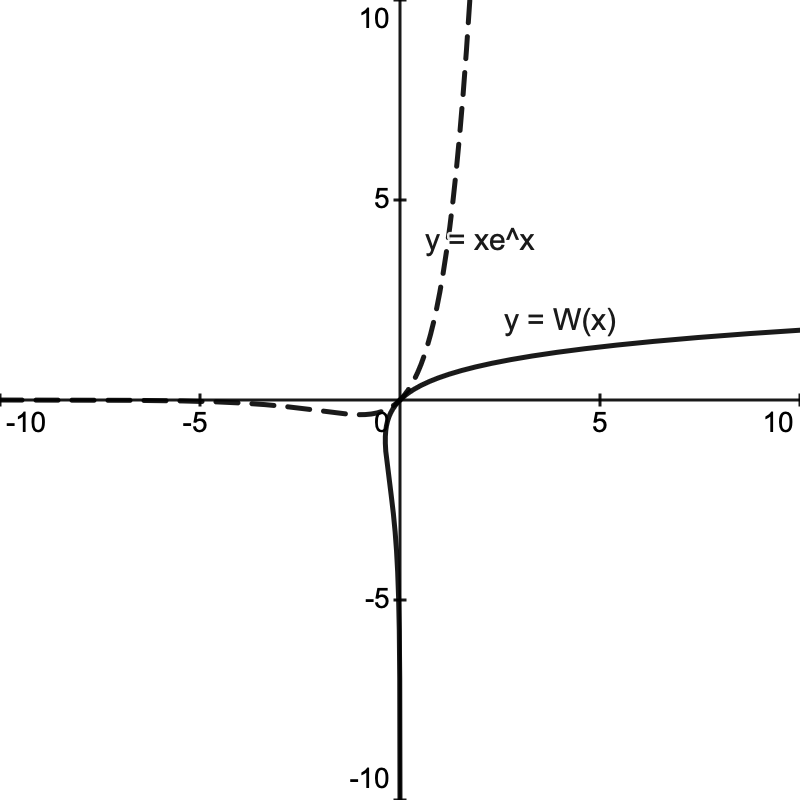
\includegraphics[width=0.5\textwidth]{fig1}
	\caption{Graph of the Lambert $W$ function and its inverse.}
\end{figure}
\pagebreak
\noindent This function has many applications to biology, chemistry, and physics. For example, it is used to find the flight time of a projectile experiencing small air resistance. The \textbf{inverse function theorem} is a tool used to study the derivatives of an inverse function when we understand the derivatives of the original function.

\section{Inverse Function Example}
Consider the curve \[y = x^2+1\] The derivative with respect to $x$ is \[\frac{dy}{dx} = 2x\] To find the curve representing the inverse, solve for $x$ in terms of $y$. This curve is represented by the equation \[\sqrt{y-1} =x\] Instead of switching the variables $x$ and $y$, it is better to \textbf{think of the inverse as a function taking in y values and outputting x values.} The derivative with respect to $y$ is \[\frac{dx}{dy} = \frac{1}{2\sqrt{y-1}} = \frac{1}{2x}\] Looking back at the derivative of the original function, it is apparent that \[\frac{dx}{dy} = \frac{1}{\left(\frac{dy}{dx}\right)}\] This relationship holds in general and is called the \textbf{Inverse Function Theorem} in one variable. Observe that the relationship between the derivative of the function and the derivative of the inverse function fails when the derivative is 0. 

\section{Inverse Function Theorem}
Let $(a,b)$ be a point on the curve $y = f(x)$ such that $f'(a) \neq 0$. The inverse function will take the form $x = f^{-1}(y)$. Then, \[\frac{df^{-1}}{dy}(b) = \frac{1}{\frac{df}{dx}(a)}\] If $g(y) = f^{-1}(y)$, then the Inverse Function Theorem can be reformulated as \[g'(b) = \frac{1}{f'(a)}\]

\textbf{Note that the derivative of the inverse function is evaluated at the y coordinate while the derivative of the original function is being evaluated at the x coordinate.}

\begin{figure}[h]
	\centering
	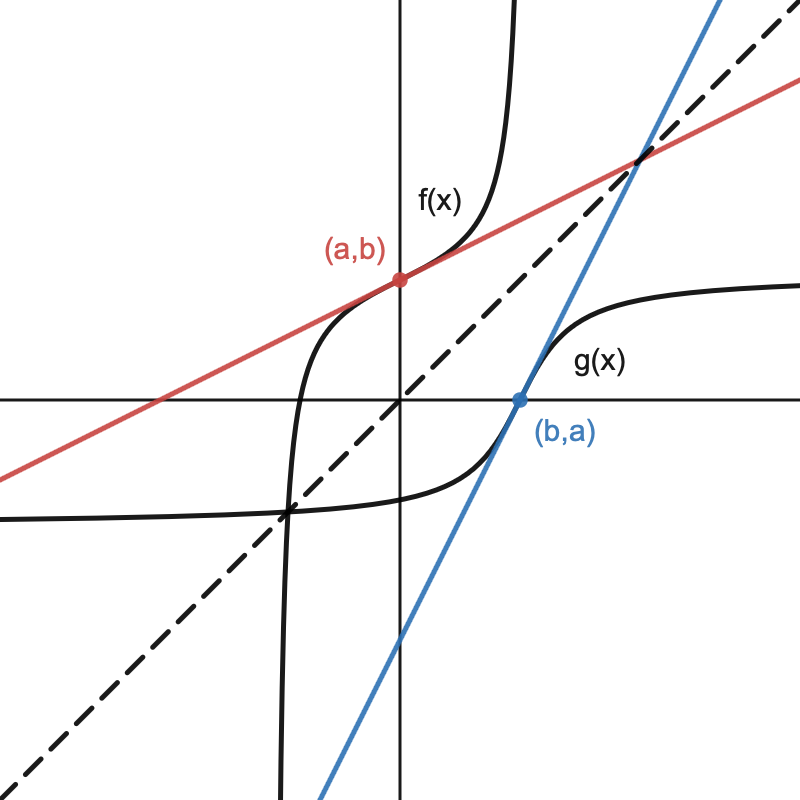
\includegraphics[width=0.5\textwidth]{fig2}
	\caption{Function and Inverse Function with Corresponding Tangent Lines.}
\end{figure}
\begin{proof}
Figure 2 depicts the function $f(x)$ and its inverse $g(x) = f^{-1}(x)$. The tangent line to the curve $y = g(x)$ at $x = b$ can be derived in two different ways. The first way is to use the fact that $g'(b)$ is the slope of the tangent line at the point $(b,a)$ Therefore,
\begin{equation}
y-a = g'(b)(x-b)
\end{equation}

The second way is to use the properties of inverses. Since the inverse function can be determined geometrically through reflection by the line $y=x$, the tangent line of the inverse function will be the inverse of the tangent line to the original function. The tangent line of the original functions has slope $f'(a)$ and passes through $(a,b)$. Therefore, 
\begin{equation}
y-b = f'(a)(x-a)
\end{equation}
Solving for the inverse relation 
\begin{equation}
y-a = \frac{1}{f'(a)}(x-b)
\end{equation}
Since equation 3.1 and equation 3.3 are both descriptions of the same line, it must be the case that \[g'(b) = \frac{1}{f'(a)}\] completing the proof.
\end{proof}

\section{Applying the Inverse Function Theorem}
\begin{center}
\begin{tabular}{|c|c|c|}
\hline
$x$ & $f(x)$ & $f'(x)$ \\
\hline
0 & 2 & 3 \\
1 & 4 & 0 \\
2 & 1 & 2 \\
3 & 6 & 5 \\
\hline
\end{tabular}
\end{center}

\noindent Consider the function $f(x)$ and its derivative $f'(x)$ described by the table above. If $g(x) = f^{-1}(x)$, the inverse function theorem implies \[g'(1) = \frac{1}{f'(2)} = \frac{1}{2}\] Similarly, $g'(2) = 1/3$ and $g'(6) = 1/5$. However, the inverse function theorem cannot be used to find $g'(4)$ since $f'(1) = 0$ Moreover, $g'(3)$ cannot be found since there is not a corresponding $x$ value on the table such that $f(x) = 3$. 

\end{document}